\chapter{Instalace a údržba}
Aplikace lze provozovat jako 2 oddělené celky, kterým můžeme říkat frontend a backend.
\section{Frontend}
Je rozhraní mezi aplikací a uživatelem, v tomto případě tedy webová aplikace běžící na Apache serveru s PHP modulem. Na stejném serveru může běžet i databáze.
\section{Backend}
Je ta část aplikace, která běží na pozadí a zajišťuje vlastní vyhotovování nahrávek. Ze serveru, kde běží backend, se také poté distribuují výsledky. Pokud bychom neměli dostatek místa, je možné aplikaci dále rozdělit na další server, který by se staral o distribuci a nahrávky by se po~uložení ukládaly na distribuční server třeba pomocí NFS sdílení. Naopak pokud budeme chtít, může běžet backend na stejném serveru jako frontend.

\begin{figure}[ht]
\begin{center}
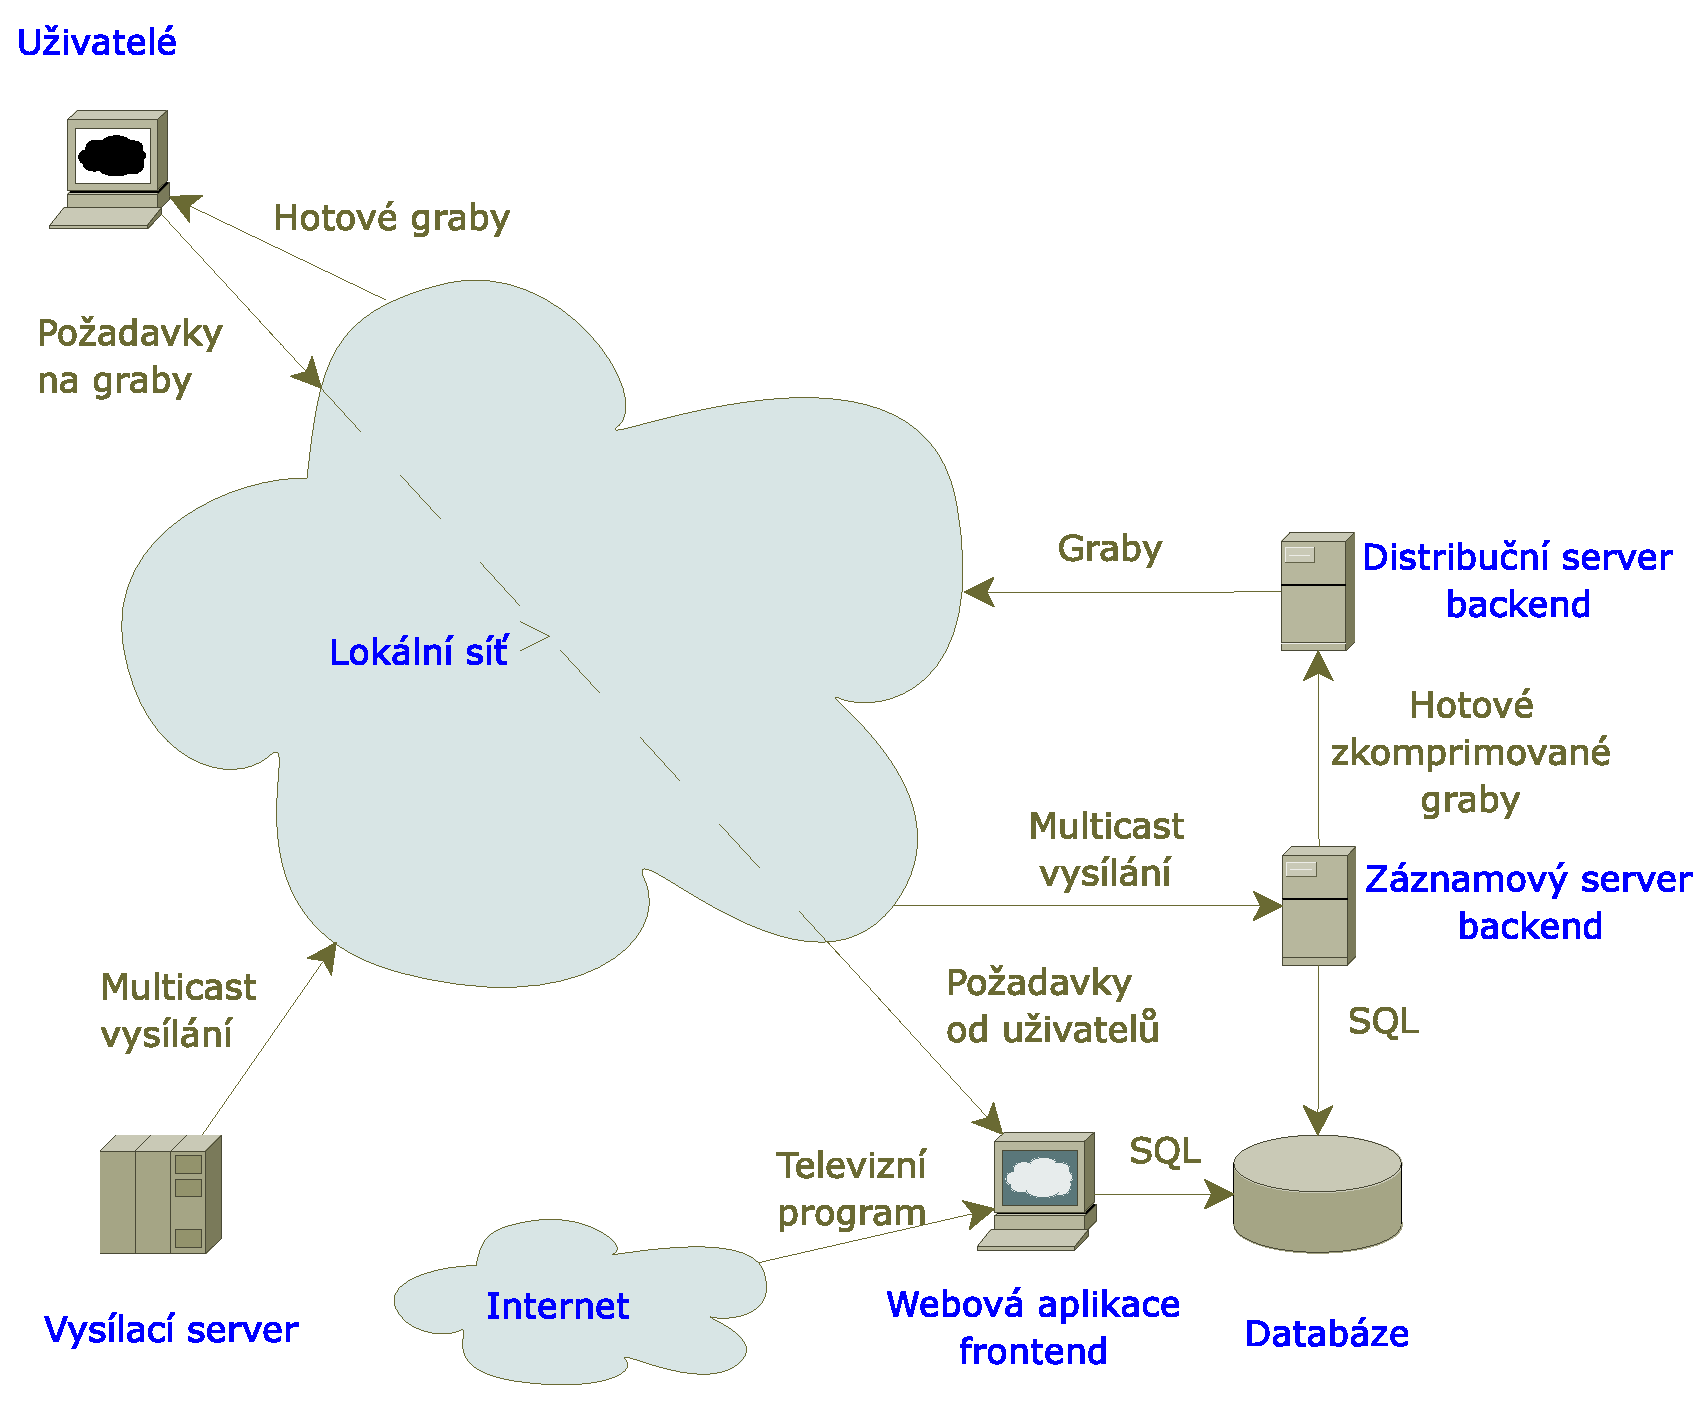
\includegraphics[width=15cm]{images/dvbgrab.eps}
\caption{Komponenty DVBgrabu}
\label{fig:dvbgrab}
\end{center}
\end{figure}

\section{Potřebné knihovny a pomocné programy}
\subsection{Apache}
Apache jako webový server budeme potřebovat jak na backend tak na frontend serveru.

Minimálně pro backend server je dobré použít buď verzi 1.x nebo až 2.2, protože verze 2.0 měla problémy se soubory většími nez 2GB, které jako graby často vznikají.
\subsection{PHP}
Na webovém serveru je potřeba modul do apache. Na záznamovém stačí PHP interpret přístupný z příkazového řádku. Obvykle instalace obsahuje oba. Aplikace byla otestována jak na PHP verze 4 tak 5. V PHP musí být povoleny některé rozšíření, viz. dále.
\subsection{php-pear-Log}
Logovací systém, obdoba log4j pro Javu. Je potřeba na obou serverech a jsou přes něj zapisovány veškeré záznamy do logovacích souborů. Logovací soubory se používají 4 a jsou v podadresáři log.
\bitem
\item\textbf{dvbgrab.log} -- obecné hlášky systému
\item\textbf{dvbgrab.log.sql} -- veškerý SQL kód, který je volán
\item\textbf{dvbgrab.log.sys} -- veškeré příkazy operačního systému, které jsou volány z PHP
\item\textbf{dvbgrab.log.clean} -- logování výstupu z údržbového skriptu.
\eitem

Logování SQL a systémových příkazů může generovat poměrně velké logy, proto by mělo být po odladění aplikace vypnuto v dolib.inc.php.
\subsection{php-json}
Podpora pro JSON (JavaScript Object Notation) do PHP. JSON je použit pro dotazy na detail televizního pořadu nebo grabu v seznamu grabů. Je to alternativní notace, která je vrácena na~volání XMLHttpRequestu z javascriptu. Toto rozšíření usnadňuje generování JSON odpovědi ve skriptu, který z databáze detail načítá a zpracování přijaté odpovědi ve webové stránce.
\subsection{php-adodb}
Knihovna pro abstraktní přístup k různým databázím. Všechna volání do databáze překládá ze~své syntaxe do syntaxe použitého databázového stroje.
\vfil
\pagebreak
\subsection{XMLTV}
Pokud chcete použít XMLTV modul pro načítání televizního programu, bude potřeba nainstalovat tento balík. Buď v něm přímo najdete stahovací skript pro požadované programy, nebo se bude hodit alespoň skript tv\_sort.
\subsection{Databáze}
DVBgrab by měl fungovat s libovolnou databází, která je podporována v ADOdb. Otestovaný je na PostgreSQL a MySQL, také skripty pro založení databáze jsou připraveny v syntaxi pro~MySQL a PostgreSQL.
\section{Stažení DVBgrabu}
DVBgrab je dostupný na na sourceforge.net. K dispozici jsou jak jednotlivé uveřejněné verze, tak čtení z vývojového repozitáře subversion.

Odkaz na jednotlivé verze naleznete na stránkách projektu http://dvbgrab.sourceforge.net/.

Pro export z repozitáře subversion použijte následující:

Starší verze \textbf{dvbgrab-1.0}
\begin{small}\begin{verbatim}
svn export --username anonymous \
https://dvbgrab.svn.sourceforge.net/svnroot/dvbgrab/tags/dvbgrab-1.0 dvbgrab
\end{verbatim}\end{small}
Aktuální verze \textbf{dvbgrab-2.0}
\begin{small}\begin{verbatim}
svn export --username anonymous \
https://dvbgrab.svn.sourceforge.net/svnroot/dvbgrab/tags/dvbgrab-2.0 dvbgrab
\end{verbatim}\end{small}
\textbf{Vývojová verze}
\begin{small}\begin{verbatim}
svn export --username anonymous \
https://dvbgrab.svn.sourceforge.net/svnroot/dvbgrab/trunk dvbgrab
\end{verbatim}\end{small}

\section{Založení databáze}

V podadresáři sql jsou připraveny skripty convert.sh, mysql.sql, postgres.sql, data.sql.
\bitem
\item\textbf{convert.sh} -- je pro konverzi databázových dat z dvbgrab-1.0 na dvbgrab-2.0, přesto tato konverze není doporučena a je bezpečnější převést pouze uživatelské účty. Obě verze DVBgrabu nechat spuštěné nějakou dobu paralelně (starý DVBgrab nechat dostupný třeba pod jiným názvem) a aktuální požadavky nechat vyřešit v původní verzi a až budou zpracovány, tak starou verzi zrušit a ponechat pouze novou
\item\textbf{mysql.sql} -- založí všechny potřebné tabulky pro DVBgrab na MySQL
\item\textbf{postgres.sql} -- založí všechny potřebné tabulky pro DVBgrab na PostgreSQL
\item\textbf{data.sql} -- do tabulek vloží několik výchozích záznamů. 
\eitem

Do tabulky param vloží datum poslední aktualizace uživatelských účtů (někdy v minulosti). 

Do tabulky tvgrabber přidá dva záznamy skriptů na stahování televizního programu. Tyto záznamy lze dále upravovat přes webové konfigurační rozhraní, ale můžeme je upravit již tady. Minimálně by bylo dobré zvolit nějaké náhodné časy spouštění v cronu, aby se všechny instalace DVBgrabu nepřipojovaly na servery s programem současně. Do tabulky encoder přidá pět záznamů, jeden pro MPEG-2 a čtyři pro MPEG-4 s různě velkým rozlišením záznamu. 

Pak do channel přidá televizní kanály (ČT1, ČT2, Nova, Prima). Zde je dobré zkontrolovat IP adresy a porty, ze kterých má systém dané kanály ukládat a také se ujistit, že případný xmltv modul používá stejné ID kanálu jako je v této tabulce. Pokud přidáváme nový kanál, tak určíme také název souboru s logem a logo uložíme do adresáře images.

Nakonec do tabulky news můžeme přidat několik zpráv uživatelům, které se budou zobrazovat ve webovém rozhraní v sekci novinky.

\section{Konfigurace DVBgrabu}

Stažený adresář uložíme na webový server do zvolené cesty (např: /var/www/dvbgrab). U webového serveru apache můžeme nastavit virtuální server, který pak adresář s DVBgrabem uveřejní pod jinou URL, než je název serveru, takže třeba http://dvbgrab.domena.cz.

Jako výchozí použijeme distribuční konfigurační soubor config.php.dist, který překopírujeme jako config.php.
Zkontrolujeme, že odkaz ADOdb ukazuje na knihovnu php-adodb, případně upravíme cíl odkazu, aby odpovídal umístění naší ADOdb (podle distribuce).

Chceme-li použít webové konfigurační rozhraní, je třeba nastavit právo na zápis i pro uživatele, pod kterým běží webový server. To můžeme zajistit spuštěním skriptu configure.sh. Nyní již můžeme začít používat administrační rozhraní, které by mělo být dostupné na URL\linebreak[4] http://dvbgrab.domena.cz/setup.php. Případně můžeme vše nastavit přímo editací souboru config.php.

Podrobnější popis jednotlivých voleb konfiguračního souboru:
\bitem
\item\textbf{db\_name} -- Určuje název databáze, kterou jsme pro DVBgrab založili.
\item\textbf{db\_type} -- Určuje typ databázového serveru, jeden z (access, ado, ado\_access, ado\_ms-sql, db2, odbc\_db2, vfp, fbsql, ibase, firebird, borland\_ibase, informix, informix72, ldap, mssql, mssqlpo, mysql, mysqlt, maxsql, oci8, oci805, oci8po, odbc, odbc\_mssql, odbc\_oracle, odbtp, odbtp\_unicode, netezza. pdo, postgres, postgres64, postgres7, postgres8, sapdb, sqlanywhere, sqlite, sqlitepo, sybase, sybase\_ase).
\item\textbf{db\_host} -- Jméno počítače, na kterém běží databáze.
\item\textbf{db\_user} -- Jméno databázového uživatele.
\item\textbf{db\_pass} -- Heslo pro přístup do databáze.
\item\textbf{auth\_db\_used} -- Určuje, zda uživatelé budou mít možnost používat heslo z nějaké jiné externí databáze. To znamená, že pokud máme třeba databázi uživatelů lokální sítě a v~ní již hesla pro nějaké jiné služby, tak můžeme ověřovat uživatele tam.

Registrace poté ověří, zda takový uživatel existuje v externí databázi. Pokud existuje, musí zadat stejné heslo, jako má uživatel zvoleného jména v externí databázi. Pokud zadá správné, může být zaregistrován a v databázi DVBgrabu je pak místo jeho hesla uloženo pouze slovo \quotedblbase extern'', které značí, že uživatel využívá externí heslo. Pokud heslo neodpovídá externí databázi, je registrace zamítnuta. Pokud uživatel s daným jménem v~externí databázi neexistuje, registrace může být provedena a heslo se ukládá do databáze DVBgrabu. Hodnota 1 znamená používat externí databázi, hodnota 0 nepoužívat.

Pro uživatele s externím heslem také platí omezení, že nelze přes DVBgrab měnit heslo a~ani si poslat nově vygenerované v případě jeho zapomenutí (to by měly řešit systémy nad externí databází).
\item\textbf{auth\_db\_used\_only} -- Určuje, zda se mohou zaregistrovat a používat DVBgrab i jiní uživatelé, než ti s externím heslem. Tím můžeme omezit DVBgrab jen na uživatele, kteří jsou registrováni v naší externí databázi (třeba pouze registrovaní uživatelé lokální sítě). Hodnota 1 znamená pouze ti s externím heslem, hodnota 0 i jiní.
\item\textbf{auth\_db\_name} -- Název externí databáze v databázovém stroji.
\item\textbf{auth\_db\_type} -- Typ databáze pro externí ověřování, může nabývat stejných hodnot jako db\_type.
\item\textbf{auth\_db\_host} -- Jméno počítače, na kterém běží databáze externího ověřování.
\item\textbf{auth\_db\_user} -- Jméno databázového uživatele s přístupem do externí databáze.
\item\textbf{auth\_db\_pass} -- Heslo tohoto uživatele pro přístup do databáze.
\item\textbf{auth\_db\_select} -- SQL dotaz na ověření hesla uživatele, v tomto řetězci se nahradí dva textové řetězce dvbgrab\_username je nahrazeno zadaným uživatelským jménem \linebreak[4] a dvbgrab\_password je md5 zadaného hesla. Pokud tento select vrátí alespoň jeden řádek, uživatelské jméno a heslo je přijato.
\item\textbf{auth\_db\_user\_select} -- SQL dotaz na uživatele, jestli existuje v externí databázi. V~tomto řetězci se nahradí pouze dvbgrab\_username. Pokud se vrátí alespoň jeden řádek, uživatel v externí databázi existuje. Vrácené řádky by měly mít strukturu uživatelské jméno, heslo v MD5, uživatelský e-mail, ip adresa. Pokud nějaké sloupce nemůžeme podle externí databáze určit, vrátíme v odpovídajícím sloupci NULL.
\item\textbf{error\_status} -- Množství informací o vzniklé chybě:
\bitem
\item 0 -- Každá chyba je vypsána do stránky.
\item 1 -- Každá chyba je odeslána na chybový e-mail.
\item 2 -- Každá chyba je ignorována. Toto je výchozí nastavení.
\eitem
\item\textbf{error\_email} -- E-mail, kam budou odesílány informace o chybách webového rozhraní.
\item\textbf{admin\_email} -- E-mail, kam budou odesílány informace o chybách v grabovacím systému a ze kterého budou e-maily chodit uživatelům.
\item\textbf{report\_email} -- E-mail, kam bodou odesílány souhrné informace o využití systému.
\item\textbf{proxy\_server} -- IP adresa HTTP proxy serveru, pokud musí být použit pro přístup k~vnějším www stránkám (pro stahovače televizního programu).
\item\textbf{proxy\_port} -- Port pro HTTP proxy.
\item\textbf{grab\_history} -- Kolik dnů se mají uchovávat nagrabované pořady pro stažení.
\item\textbf{tv\_days} -- Na kolik dnů dopředu se má načítat televizní program.
\item\textbf{midnight} -- Kterou hodinu budeme považovat za půlnoc při rozdělování pořadů do jednotlivých dnů. (Televizní den potom chápeme například od šesté hodiny ranní do šesté hodiny další den.
\item\textbf{hour\_frac\_item} -- Do jak velikých úseků budeme seskupovat seznam pořadů. 24 by mělo být dělitelné hodnotou beze zbytku. To umožňuje vertikální zarovnavaní všech televizních kanálů.
\item\textbf{grab\_quota} -- Kolik grabů může zadat uživatel týdně.
\item\textbf{user\_inactivity\_limit} -- Po kolika dnech neaktivity bude uživatelský účet zrušen.
\item\textbf{dvbgrab\_log} -- Do jakého souboru se mají ukládat informace o průběhu grabování.
\item\textbf{grab\_date\_start\_shift} -- O kolik minut se má posunout začátek nahrávání pořadu, proti plánovanému začátku televizního pořadu.
\item\textbf{grab\_date\_stop\_shift} -- O kolik minut se má posunout konec nahrávání pořadu, proti plánovanému konci televizního pořadu.
\item\textbf{record\_time\_after\_last} -- Jak dlouho nahrávat zvolený pořad, pokud neznáme následující (třeba poslední pořad v noci má následující až druhý den ráno). Zadáváme v~sekundách.
\item\textbf{hostname} -- Název počítače, ze kterého distribuujeme hotové nahrávky. Případně to může být i celá úvodní část URL (pokud nemáme virtuální host v apache nastaven do~uživatelského adresáře). Nekončí lomítkem, takže např: \quotedblbase http://grab.domena''.
\item\textbf{grab\_storage} -- Adresář, do kterého se budou nahrávat pořady. Je to sdílený adresář všech uživatelů. Nekončí lomítkem.
\item\textbf{grab\_storage\_size} -- Kolik GB prostoru máme vyhrazeno pro nahrané pořady. (Omezení velikosti pro adresář grab\_storage).
\item\textbf{grab\_storage\_min\_size} -- Minimální množství volného místa na grabovacím disku, při kterém začneme promazávat starší graby.
\item\textbf{grab\_root} -- Adresář, kam se budou ukládat odkazy na hotové pořady. Musí být přístupný pro http server. V tomto adresáři se budou zakládat uživatelské adresáře. Nekončí lomítkem.
\item\textbf{grab\_backend\_lang} -- Jazyk používaný v backend skriptech (cz, sk, en, fr, ..). Tento se použije pouze v případě, že se zpráva posílá správci DVBgrabu nebo uživateli, který nemá jestě uložen svůj naposledy použitý jazyk.
\item\textbf{grab\_backend\_strip\_diacritics} -- Příznak, zda se má z nahraných souborů odstraňovat diakritika, nebo jestli součástí názvu nahrávky je pouze ID číslo záznamu. Diakritika na některých souborových systémech nemusí být podporována nebo nastavena na UTF-8, ve kterém máme názvy pořadů. Proto se používá odstranění diakritiky, které ale nelze vyřesit úplně univerzálně pro všechny znaky z UTF-8. Pro češtinu funguje dobře, v čínštině by bylo lepší použít jen ID. Název pořadu včetně diakritiky pak máme v přidruženém, popisném XML souboru. Hodnota 0 určuje použití ID, hodnota 1 název pořadu.
\eitem

V poslední části je definice stahovačů televizního programu. Předdefinované můžeme povolovat nebo zakazovat. Také můžeme definovat nový. Každý stahovač má 3 důležité parametry:

\bitem
\item\textbf{tvg\_name} -- Jméno stahovače.
\item\textbf{tvg\_cron\_time} -- Čas naplánovaného spouštění pomocí cron démona. Zadává se přímo syntaxe cronu, tzn. 5 čísel udávajících v pořadí minutu, hodinu, den v měsíci, měsíc, den v týdnu. Místo čísla můžeme použít buď hvězdičku (značí, že na daném údaji nezáleží) nebo */N, kde N určuje násobek jednotky, ve které se příkaz má spoustět (*/5 u minut znamená každý celý násobek 5 minut). Hodnota \quotedblbase 0 23 * * 6'' potom znamená, že se stahovač má spouštět každou sobotu, v 23:00. Tyto údaje volíme nejlépe na nějakou noční dobu, kdy servery poskytovatele nebudou tolik zatíženy. Také se je snažíme volit pokud možno náhodně, aby se minimalizovala pravděpodobnost, že všechny instalace DVBgrabu stahují ze stejných serverů ve stejný okamžik.
\item\textbf{tvg\_cron\_cmd} -- Příkaz, který má cron démon spouštět. Obvykle bude začínat nastavením pracovního adresáře ke stahovacím skriptům, aby stahovací skripty mohli načítat pomocné knihovny z DVBgrabu na základě jejich relativních cest.
\eitem
\pagebreak
Pokud jsme s konfigurací již spokojeni, použijeme tlačítko \quotedblbase Nastavit''. To aktualizuje soubor config.php a vypíše nám informaci o aktuální konfiguraci pro cron démon. V té nahradíme \quotedblbase BACKEND\_DIR'' za skutečný adresář, odkud budou spouštěny backend skripty a daný výpis si zkopírujeme do schránky. Na záznamovém serveru použijeme příkaz crontab -e na editaci konfigurace cron démona a vložíme text ze schránky. Tím máme zajištěno pravidelné volání údržbového skriptu, zasílání informací o využívání DVBgrabu a spouštění stahovačů televizního programu.

Pokud máme záznamový server zvlášť, je potřeba přesunout adresář backend tam. To je nejlepší udělat pomocí archivátoru tar, který nám symbolické odkazy z adresáře backend na sdílené soubory nahradí jejich skutečnou kopií. Vzniklý archiv tar pak rozbalíme na cílovém serveru a podadresář adodb buď nahradíme správným symbolickým odkazem nebo ponecháme ten nakopírovaný z prvního serveru.

Automatické spouštění DVBgrabu při startu systému zajišťuje skript service/dvbgrab, který upravíme podle aktuálního umístění skriptu dvbgrab\_service a nakopírujeme do adresáře podle distribuce (např. /etc/init.d/dvbgrab). Poté stačí naplánovat, ve kterých runlevelech se má služba spouštět a kde zastavovat.

\section{The maintainance of recording server}
The maintainance is performed by automatically started script clean.php.

\subsection{Removing inactive users}
Removes users, who didn't sign up to DVBgrab in period of several days (wrt. config option user\_inactivity\_limit) and they didn't request anything. This will provide removing user and releasing his IP address after his moving from the dorm (unless he uses himself the function for immediate removing his account in advance). It removes also all his requests and his user's address book. An e-mail with information about the removing account will be delivered to the user.

\subsection{Users' accounts updating}
When the user changes the password or distributing IP address, new date of the last change is set in database. This script will always regenerate .htaccess files with every start for all users, who changed their settings between the last running of the script and actual time. Then it will move date of the last updating to the actual time.

\subsection{Control of unknown users' accounts}
Script will control, if there is appropriate database user for all directories, if not, they can be removed, eventually at least printed on the screen.

\subsection{Removing needless .ts files}
All records are saved to the file with .ts extension. With every start of the script these files are controlled, if there exists any unsatisfied request for encoding. If not, .ts file is removed. If yes, it is written to the log file, which format is missing yet to prepare.

\subsection{Control of free space}
In records directory an amount of used space and free space is watched. 

The oldest records start to be removed, if maximum enabled size of records directory is exceeded (wrt. grab\_storage\_size) or if there is less free space than configurated constant (grab\_storage\_min\_size).     

If it is necessary to remove also the records, which are finished for shorter time than planned records keeping (grab\_history), a warning e-mail is sent to admin.

\subsection{Removing old data}
In a database we don't need to keep television program, that is several years old and it is good to display on the web also the finished records after removing. That's why only data older than three times the period for keeping records (3 x grab\_history days) are removed from database. Users' requests are removed as well as format requests, own records and television program.

\section{The manual maintainance of users}
Sometimes it is necessary to remove manually those users, who e.g. move from the dorm and don't remove their accounts. If their IP address is given to a new user, who would like to register in DVBgrab before the period for automatic removing original account is exceeded by reason of inactivity, then registration fails by reason of IP conflict. In these cases the best solution is to set manually a date of the last activity of original account e.g. a year ago, and so removing account is provided by the maintainance script, including removing his address book and sending informational e-mail.

For spamming of registered users script backend/send\_user\_info.php might be used, in which we modify the text of the message and by its start we send the message including sign up data to every user of DVBgrab. This is suitable to use e.g. after the conversion of the database from DVBgrab version 1 to version 2, when the changes in the rules for characters in users names were performed.

\section{The maintainance of backend scripts}
Every start and stop of recording or encoding loops should be provided by script dvbgrab\_service, which is a component of installation package. In this script we check the path to backend directory.

Script dvbgrab\_service supports these parameters:
\bitem
\item \textbf{start} -- starts recording and encoding loop
\item \textbf{startg} -- starts only recording loop
\item\textbf{starte} -- starts only encoding loop
\item\textbf{stop} -- stops both loops
\item\textbf{stopg} -- stops only recording loop
\item\textbf{stope} -- stops only encoding loop
\item\textbf{restart} -- restarts both loops
\item\textbf{restartg} -- restarts only recording loop
\item\textbf{restarte} -- restarts only encoding loop
\item\textbf{status} -- shows, if the loops are still running. Then the list of records (which are in the queue and also those which are just saved) is shown for every encoding format.
\eitem

Stopping of encoding loop is supplemented with restoring of the queue for encoding (by the script backend/encode\_queue\_restore.php). It means that after stop of the loop request status returns from status \quotedblbase Encoding'' to status \quotedblbase Ready'', so they can be queued again after restart of the loop.

Displaying the queue for encoding and currently saved records can be provided also manually by means of the script backend/encode\_queue\_print.php.

We have startup script for operating system (/etc/init.d/dvbgrab), which uses dvbgrab\_service when starting and stopping DVBgrab as system service.

